% ============================================================================
% HELEN OS — Constitutional Regime Diagram (standalone figure)
%
% Compilation: pdflatex helen_os_regime_diagram.tex
%              lualatex helen_os_regime_diagram.tex
%
% For inclusion in paper:
%   \begin{figure}[h]
%     \input{helen_os_regime_diagram_body.tex}
%     \caption{...}
%     \label{fig:regimes}
%   \end{figure}
%
% Frozen: 2026-03-14  authority=NONE
% ============================================================================

\documentclass[tikz, border=10pt]{standalone}

\usepackage{tikz}
\usetikzlibrary{arrows.meta, positioning, calc}
\usepackage{amsmath}
\usepackage[T1]{fontenc}

\begin{document}
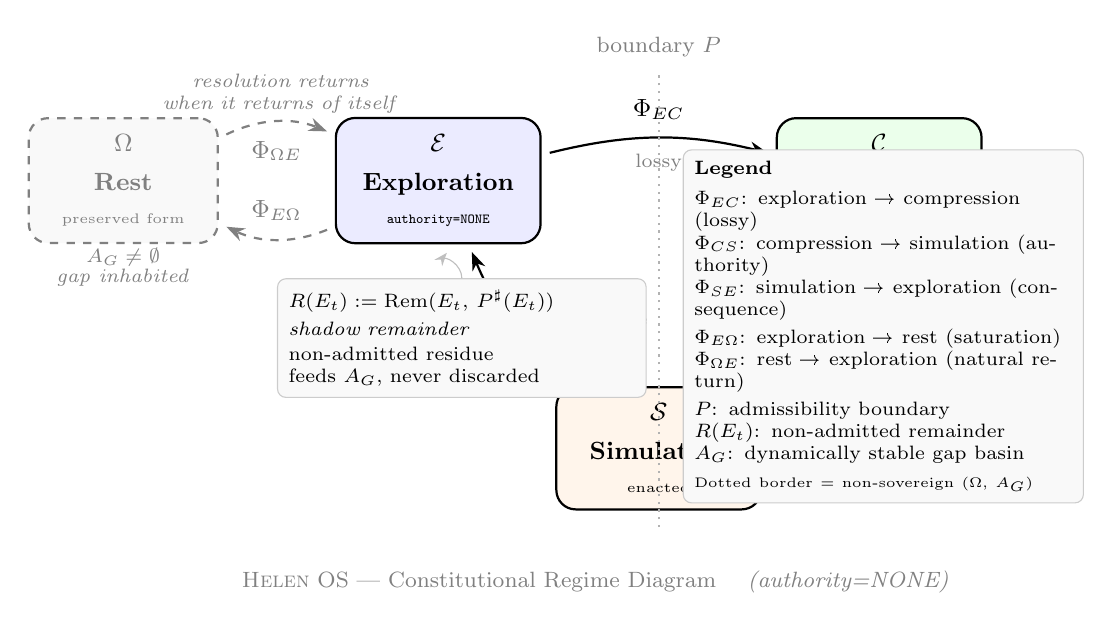
\begin{tikzpicture}[
  >=Stealth,
  every node/.style={font=\small},
  %% ── Regime node styles ──────────────────────────────────────────────────
  regime/.style={
    draw, rounded corners=7pt,
    minimum width=2.6cm, minimum height=1.3cm,
    align=center, thick, inner sep=6pt
  },
  omega/.style={
    draw, dashed, rounded corners=7pt,
    minimum width=2.4cm, minimum height=1.3cm,
    align=center, thick, inner sep=6pt, gray
  },
  %% ── Arrow styles ────────────────────────────────────────────────────────
  arr/.style={
    ->, thick, shorten >=3pt, shorten <=3pt
  },
  arrg/.style={
    ->, thick, gray, dashed, shorten >=3pt, shorten <=3pt
  },
  %% ── Annotation styles ───────────────────────────────────────────────────
  ann/.style={font=\scriptsize, align=left, text=gray!80},
  boxann/.style={
    draw=gray!40, rounded corners=3pt, fill=gray!5,
    font=\scriptsize, align=left, inner sep=4pt
  },
]

%% ═══════════════════════════════════════════════════════════════════════════
%% NODES
%% ═══════════════════════════════════════════════════════════════════════════

%% — Three main regimes ──────────────────────────────────────────────────────
\node[regime, fill=blue!8]
  (E) at (0, 4.2)
  {$\mathcal{E}$\\[3pt]\textbf{Exploration}\\[1pt]{\tiny\texttt{authority=NONE}}};

\node[regime, fill=green!8]
  (C) at (5.6, 4.2)
  {$\mathcal{C}$\\[3pt]\textbf{Compression}\\[1pt]{\tiny ledger-bound}};

\node[regime, fill=orange!8]
  (S) at (2.8, 0.8)
  {$\mathcal{S}$\\[3pt]\textbf{Simulation}\\[1pt]{\tiny enacted}};

%% — Omega regime ────────────────────────────────────────────────────────────
\node[omega, fill=gray!5]
  (Om) at (-4.0, 4.2)
  {$\Omega$\\[3pt]\textbf{Rest}\\[1pt]{\tiny preserved form}};

%% — Gap basin A_G inside Omega ──────────────────────────────────────────────
\node[font=\scriptsize, gray, align=center]
  at (-4.0, 3.1)
  {$A_G \neq \emptyset$\\[-1pt]\emph{gap inhabited}};

%% ═══════════════════════════════════════════════════════════════════════════
%% MAIN PRODUCTION CYCLE
%% ═══════════════════════════════════════════════════════════════════════════

\draw[arr, bend left=14]
  (E) to
    node[above, yshift=3pt]        {$\Phi_{EC}$}
    node[below, yshift=-2pt, gray] {\scriptsize lossy}
  (C);

\draw[arr, bend left=14]
  (C) to
    node[right, xshift=3pt]        {$\Phi_{CS}$}
    node[left,  xshift=-3pt, gray] {\scriptsize authority}
  (S);

\draw[arr, bend left=14]
  (S) to
    node[left,  xshift=-3pt]       {$\Phi_{SE}$}
    node[right, xshift=3pt, gray]  {\scriptsize consequence}
  (E);

%% ═══════════════════════════════════════════════════════════════════════════
%% OMEGA SUSPENSION BRANCH
%% ═══════════════════════════════════════════════════════════════════════════

\draw[arrg, bend left=24]
  (E) to
    node[above, yshift=3pt] {\small $\Phi_{E\Omega}$}
  (Om);

\draw[arrg, bend left=24]
  (Om) to
    node[below, yshift=-3pt] {\small $\Phi_{\Omega E}$}
  (E);

%% — "resolution returns of itself" label ───────────────────────────────────
\node[font=\scriptsize, gray, align=center, text width=3.2cm]
  at (-2.0, 5.3)
  {\emph{resolution returns\\when it returns of itself}};

%% ═══════════════════════════════════════════════════════════════════════════
%% ADMISSIBILITY BOUNDARY P
%% ═══════════════════════════════════════════════════════════════════════════

\draw[thick, dotted, gray!60]
  (2.8, -0.2) -- (2.8, 5.6);

\node[gray, font=\footnotesize, align=center]
  at (2.8, 5.9)
  {boundary~$P$};

%% ═══════════════════════════════════════════════════════════════════════════
%% SHADOW REMAINDER R(E_t)
%% ═══════════════════════════════════════════════════════════════════════════

\node[boxann, text width=4.4cm]
  (Rbox) at (0.3, 2.2)
  {$R(E_t) := \operatorname{Rem}(E_t,\, P^{\sharp}(E_t))$\\[2pt]
   \emph{shadow remainder}\\[1pt]
   non-admitted residue\\
   feeds $A_G$, never discarded};

\draw[->, gray!50, thin, shorten >=4pt]
  (Rbox.north) to[out=90, in=230] ($(E.south) + (0.2, 0)$);

%% ═══════════════════════════════════════════════════════════════════════════
%% LEGEND
%% ═══════════════════════════════════════════════════════════════════════════

\node[boxann, anchor=south east, text width=4.8cm]
  at (8.2, 0.1)
  {\textbf{Legend}\\[3pt]
   $\Phi_{EC}$: exploration → compression (lossy)\\
   $\Phi_{CS}$: compression → simulation (authority)\\
   $\Phi_{SE}$: simulation → exploration (consequence)\\[2pt]
   $\Phi_{E\Omega}$: exploration → rest (saturation)\\
   $\Phi_{\Omega E}$: rest → exploration (natural return)\\[2pt]
   $P$: admissibility boundary\\
   $R(E_t)$: non-admitted remainder\\
   $A_G$: dynamically stable gap basin\\[2pt]
   {\tiny Dotted border = non-sovereign ($\Omega$, $A_G$)}};

%% ═══════════════════════════════════════════════════════════════════════════
%% CAPTION ROW
%% ═══════════════════════════════════════════════════════════════════════════

\node[font=\footnotesize, gray, align=center]
  at (2.0, -0.9)
  {\textsc{Helen}~OS --- Constitutional Regime Diagram
   \quad\textit{(authority=NONE)}};

\end{tikzpicture}
\end{document}
